\chapter{Introduction to Neural Networks}

\TODO{Chapter: Introduction}

\section{Biological Neurons}

Biological neurons are electrically excitable cells that are found in almost all
animals.
These neurons can transmit and receive electrical signals to one another via
synaptic connections, which maybe either excitatory or inhibitory.
Any given neuron will be either active or inactive depending on whether or not
its input exceeds a threshold.

\begin{center}
    \begin{tikzpicture}%[x=1pt,y=1pt]
    \newlength{\rs}
    \setlength{\rs}{1.5pt}
    % Nucleus
    \fill (0\rs,0\rs) circle (2\rs);
    % Soma
    \draw[thick] (0\rs,0\rs) circle (8\rs);
    % Dendrite
    \draw[thick] ( 45:8\rs) -- ( 45:16\rs);
        \draw[thick] ( 45:16\rs) -- ++(  0:4\rs);
        \draw[thick] ( 45:16\rs) -- ++( 90:4\rs);
    \draw[thick] ( 90:8\rs) -- ( 90:24\rs);
        \draw[thick] ( 90:16\rs) -- ++( 45:4\rs);
        \draw[thick] ( 90:16\rs) -- ++(135:4\rs);
        \draw[thick] ( 90:24\rs) -- ++( 45:8\rs);
        \draw[thick] ( 90:24\rs) -- ++(135:8\rs);
    \draw[thick] (135:8\rs) -- (135:24\rs);
        \draw[thick] (135:16\rs) -- ++( 90:4\rs);
        \draw[thick] (135:16\rs) -- ++(180:4\rs);
        \draw[thick] (135:24\rs) -- ++( 90:8\rs);
        \draw[thick] (135:24\rs) -- ++(180:8\rs);
    \draw[thick] (180:8\rs) -- (180:24\rs);
        \draw[thick] (180:16\rs) -- ++(135:4\rs);
        \draw[thick] (180:16\rs) -- ++(225:4\rs);
        \draw[thick] (180:24\rs) -- ++(135:8\rs);
        \draw[thick] (180:24\rs) -- ++(225:8\rs);
    \draw[thick] (225:8\rs) -- (225:24\rs);
        \draw[thick] (225:16\rs) -- ++(180:4\rs);
        \draw[thick] (225:16\rs) -- ++(270:4\rs);
        \draw[thick] (225:24\rs) -- ++(180:8\rs);
        \draw[thick] (225:24\rs) -- ++(270:8\rs);
    \draw[thick] (270:8\rs) -- (270:24\rs);
        \draw[thick] (270:16\rs) -- ++(225:4\rs);
        \draw[thick] (270:16\rs) -- ++(315:4\rs);
        \draw[thick] (270:24\rs) -- ++(225:8\rs);
        \draw[thick] (270:24\rs) -- ++(315:8\rs);
    \draw[thick] (315:8\rs) -- (315:16\rs);
        \draw[thick] (315:16\rs) -- ++(270:4\rs);
        \draw[thick] (315:16\rs) -- ++(360:4\rs);
    % Axon
    \draw[thick] (8\rs,0\rs) -- (12\rs,0\rs);
    \draw[thick,rounded corners=3\rs] (12\rs,-3\rs) rectangle (24\rs,3\rs);
        \fill (18\rs,0\rs) circle (1.5\rs);
    \draw[thick] (24\rs,0\rs) -- (26\rs,0\rs);
    \draw[thick,rounded corners=3\rs] (26\rs,-3\rs) rectangle (38\rs,3\rs);
        \fill (32\rs,0\rs) circle (1.5\rs);
    \draw[thick] (38\rs,0\rs) -- (40\rs,0\rs);
    \draw[thick,rounded corners=3\rs] (40\rs,-3\rs) rectangle (52\rs,3\rs);
        \fill (46\rs,0\rs) circle (1.5\rs);
    \draw[thick] (52\rs,0\rs) -- (54\rs,0\rs);
    \draw[thick,rounded corners=3\rs] (54\rs,-3\rs) rectangle (66\rs,3\rs);
        \fill (60\rs,0\rs) circle (1.5\rs);
    \draw[thick] (66\rs,0\rs) -- (68\rs,0\rs);
    \draw[thick,rounded corners=3\rs] (68\rs,-3\rs) rectangle (80\rs,3\rs);
        \fill (74\rs,0\rs) circle (1.5\rs);
    % Axon terminal
    \draw[thick] (80\rs,0\rs) -- (82\rs,0\rs);
        \draw[thick] (82\rs,0\rs) -- (86\rs,4\rs);
            \draw[thick] (86\rs,4\rs) -- (86\rs,7\rs);
            \draw[thick] (86\rs,4\rs) -- (89\rs,4\rs);
        \draw[thick] (82\rs,0\rs) -- (86\rs,-4\rs);
            \draw[thick] (86\rs,-4\rs) -- (86\rs,-7\rs);
            \draw[thick] (86\rs,-4\rs) -- (89\rs,-4\rs);
    % Labels
    % Soma
    \draw[latex'-] (65:9\rs) -- (65:36\rs);
    \node[anchor=south west,inner sep=1\rs] at (65:36\rs) {Soma};
    % Nucleus
    \draw[latex'-] (-65:3\rs) -- (-65:36\rs);
    \node[anchor=north west,inner sep=1\rs] at (-65:36\rs) {Nucleus};
    % Dendrite
    %\draw[latex'-] (225:25\rs) -- (225:36\rs);
    \draw[latex'-] (-17.7\rs,-25.7\rs) -- (-30\rs,-38\rs);
    \node[anchor=north east,inner sep=1\rs] at (-30\rs,-38\rs) {Dendrite};
    % Axon
    \draw[decorate,decoration={brace,raise=5\rs,amplitude=4\rs}] (12\rs,0\rs) -- (80\rs,0\rs);
    \node[anchor=south,inner sep=1\rs] at (46\rs,9\rs) {Axon};
    % Axon Terminal
    \draw[latex'-] (87\rs,8\rs) -- (95\rs,16\rs);
    \node[anchor=south west,inner sep=1\rs] at (95\rs,16\rs) {Axon Terminal};
\end{tikzpicture}

    \captionof{figure}{Diagram of a biological neuron.}
\end{center}

Signals are received by the neuron via connections to dendrites and soma.
If the threshold is met, electrical signals are sent along the axon to the
terminal, where it is connected to other neurons, or to a controllable cell such
as a neuromuscular junction.

\TODO{Section: Biological Neurons}

\section{Artificial Intelligence}

The idea of artificial beings capable of human intelligence can be traced back
to mythical stories from ancient Greece.
One such story was that of a mythical automaton called Talos, who circled an
island's shores to protect it from pirates and other invaders.

In the $19^\text{th}$ century, other notions of artificial intelligence were
explored by fiction in stories such as Mary Shelley's ``Frankenstein'', and
Karel \v{C}apek's ``R.U.R.''.
Some of the fictional writings of the $20^\text{th}$ century further continued
exploring the concept in novels such as Isaac Asimov's ``I, Robot''.

Academic research into artificial intelligence began around the 1940's,
primarily due to findings in neurological research at the time.
The first explorations of artificial neural networks was done by
\cite{McCulloch:1943:Logical}, who investigated how simple logic functions
might be performed by idealised networks.
The neurons within these networks operated using some basic logic rules, applied
to a discrete time system which, can be summarised using the expression
\begin{align*}
    N(t) &= (E_1(t-1) \vee E_2(t-1) \vee \dots)
        \wedge \neg(I_1(t-1) \vee I_2(t-1) \vee \dots),
\end{align*}
where $N(t)$ is the state of a neuron at time $t$, and $E_i(t-1)$ and $I_i(t-1)$
are the states of the excitatory and inhibitory connections from the previous
time step respectively.
The result is such that the neuron will only be active if at least one
excitatory connection is active and all inhibitory connections are inactive.
The versatility of this definition is demonstrated in the following examples.
\begin{center}
    \begin{tabular}{ccc}
        SR Flip-flop & & AND Gate\\
        \begin{tikzpicture}
    [   neuron/.style=
        {   draw
        ,   regular polygon
        ,   regular polygon sides=3
        ,   shape border rotate=90
        ,   inner sep=2pt
        ,   node font=\small\ttfamily
        }
    ,   baseline=0pt
    ,   >={Stealth[scale=1.2]}
    ]
    \node[neuron] (S) at (0cm, 7mm) {S};
    \node[neuron] (R) at (0cm,-7mm) {R};
    \node[neuron] (M) at (2cm, 0cm) {M};
    \draw[->] (S) to[out=0,in=150] (M);
    \draw[-o] (R) to[out=0,in=180] (M);
    \draw[->] (M.east) .. controls (3cm,1cm) and (2cm,1cm) .. (M);
    \draw[->] (M.east) to (3cm,0cm);
\end{tikzpicture}
 & & \begin{tikzpicture}
    [   neuron/.style=
        {   draw
        ,   regular polygon
        ,   regular polygon sides=3
        ,   shape border rotate=90
        ,   inner sep=2pt
        ,   node font=\small\ttfamily
        }
    ,   baseline=0pt
    ,   >={Stealth[scale=1.2]}
    ]
    \node[neuron] (A) at (-2cm, 6mm) {A};
    \node[neuron] (B) at (-2cm,-6mm) {B};
    \node[neuron] (Af) at (0cm, 18mm) {1};
    \node[neuron] (Ab) at (0cm,  6mm) {2};
    \node[neuron] (Ba) at (0cm, -6mm) {3};
    \node[neuron] (Bf) at (0cm,-18mm) {4};
    \node[neuron] (R) at (2cm,0cm) {R};
    \draw[->] (A) to[out=0,in=240] (Af);
    \draw[->] (B) to[out=0,in=120] (Bf);
    \draw[->] (Af) to[out=0,in=120] (R);
    \draw[->] (Bf) to[out=0,in=240] (R);
    \draw[->] (A) to[out=0,in=120] (Ba);
    \draw[->] (B) to[out=0,in=240] (Ab);
    \draw[-o] (A) to[out=0,in=180] (Ab);
    \draw[-o] (B) to[out=0,in=180] (Ba);
    \draw[-o] (Ab) to[out=0,in=180] (R.west);
    \draw[-o] (Ba) to[out=0,in=180] (R.west);
\end{tikzpicture}
\\
        $\displaystyle N_M(t+1) = (N_S(t) \vee N_M(t)) \wedge\neg N_R(t)$ &
        &
        $\displaystyle N_R(t+2) = N_A(t) \vee N_B(t)$\\
    \end{tabular}
    \parbox{0.9\textwidth}{%
    \captionof{figure}{Two common logic circuits using McCullochs neurons
    where the arrows and circles indicate excitatory and inhibitory
    connections respectively.}}
\end{center}
While this model provided insight into the mechanisms by which neurons operate,
the structure was static, and incapable of learning.

McCulloch's work was later cited by psychologist \cite{Hebb:1949:Organization},
who proposed that the structure of biological neural networks was dynamic, and
that frequently repeated stimuli caused gradual development.
At the scale of neuron, it was theorised that if one neuron successfully
excited another, the connection between them would strengthen, hence
increasing the likelihood that the former would be able to excite the latter
again in the future.
His theory was supported by research conducted by himself and others that showed
that intelligence-test performance in mature patients was often unaffected by
brain operations that would have prevented development in younger patients,
which suggested that learnt stimuli are processed differently to unknown
stimuli.
This hypothesis became known as Hebbian learning.

Computer simulations applying this theory to a small network were done by
\cite{Farley:1954:Simulation}.
The actions of the network were compared to that of a servo system which must
counteract any displacements so as to maintain a steady position.
The network was trained using a set of input patterns, which were subject to
non-linear transformations.
Similar to the Hebbian theory, when the network produces the correct responses,
the active connections are strengthened.
Although the results were of little neurophysiological significance, the results
were of great use for demonstrating computational simulations, which were
considerably slower at the time.

\TODO{Section: Artificial Intelligence}

\subsection{Perceptrons}

The idea of the perceptron was originally conceived by
\cite{Rosenblatt:1958:Perceptron}, to represent a simplified model of
intelligent systems free from particularities of biological organisms, whilst
maintaining some of their fundamental properties.

The perceptron was built as a dedicated machine that consisted of a number of
photovoltaic cells, analogous to a retina, that feed into an``association
area''.
This association area contains a number of cells that each calculate a weighted
sum of the receptor values and output a signal if it exceeds a threshold.
Expressed mathematically, the output of a given association cell is given by
\begin{align*}
    A_i &= \begin{cases}
        1, & \sum_j w_{i,j}x_j > \theta\\
        0, & \text{otherwise}
    \end{cases},
\end{align*}
where $x_j$ is the value from the $j^\text{th}$ photovoltaic cell, $w_{i,j}$
is the weight of the connection between association cell $i$ and photovoltaic
cell $j$, and $\theta$ is the threshold.
These value weights were implemented using variable resistance wires that the
perceptron could adjust automatically.
The outputs from the association area are then connected to response cells,
which operate in a similar fashion to the association cells.
The activation of these response cells are the outputs of the perceptron, and
indicated the classification of the input.

Similar to \cite{Farley:1954:Simulation}, the method by which the perceptron
adjusted it weights was also based on which cells were active, and whether the
correct output was produced; except that the perceptron was also able to
``penalise'' weights when an incorrect result was outputted.

This machine was initially trained to reliably identify three different shapes:
a square, a circle, and a triangle; and did so with a better than chance
probability.
When attempting to use the perceptron for more complicated tasks, such as
character recognition, it failed to produce better than chance results.

After a decade of unsuccessful real world application attempts, a book titled
``\citetitle{Minsky:1969:Perceptrons}'' by \cite{Minsky:1969:Perceptrons}, was
released.
The book provided a rigorous mathematical analysis of the model, the results
showed that single layered, simple linear perceptron networks could not
calculate XOR predicates.
A 2017 reissue of the book contained a foreword by L\'eon Bottou, who wrote
``Their rigorous work and brilliant technique does not make the perceptron look
very good...''

Following the book's release, perceptron research effectively halted for 15
years until the first successful uses of multilayer networks by
\cite{McClelland:1986:Parallel}, which also served as a departure from the
neuron outputs being boolean values.
The multilayered structure of this new model allowed it to calculate the XOR
predicates that the single layer perceptrons could not.

The output of the units within these networks were defined by
\begin{align*}
    \Rvec{a}(t+1) &= \Rvec{F}(\Rvec{a}(t),\Rvec{net}_1(t),\Rvec{net}_2(t),...),
\end{align*}
where $\Rvec{net}_i$ is the $i^\text{th}$ propagation rule applied to the
inputs, $\Rvec{F}$ is the activation function, and $\Rvec{a}(t)$ is the
activation of the units at time step $t$.
The model usually uses a simplified version which can be summarised as
\begin{align*}
    a_i &= F\left(\sum_j w_{i,j}o_j\right),
\end{align*}
where $o_j$ is the output of unit $j$.
Hebbian learning could be performed the network by using iterative methods,
the most simple of which was given by
\begin{align*}
    \Delta w_{i,j} &= \eta\,a_i o_j,
\end{align*}
where $\eta$ is the learning rate, which is a constant.

\TODO{Subsection: Perceptrons}

\subsection{Backpropagation}

In order for a neural network to learn, it must undergo some form of
optimisation process.
For the perceptron, this process was one of positive and negative reinforcement.

In the field of control theory, an optimisation method known as gradient descent
was developed by \cite{Kelley:1960:Gradient}, in which a given function of the
system is either maximised or minimised.
This is achieved by taking partial derivatives of the function with respect to
each parameter, which gives an approximation of how the function value will
change as the parameter changes.
By evaluating the partial derivatives, multiplying them by a constant, and
adding them to their respective parameters, the parameter values can be updated.
Using these new parameter values, one can expect to improve the function value.
This can be written as
\begin{align*}
    w_i' &= w_i + \eta\Rpdiff{f}{w_i}(\Rvec{x}),
\end{align*}
where $f(\Rvec{x})$ is the function to be optimised, $w_i$ is a parameter of
$f$, $w_i'$ is the updated parameter, and $\eta$ is ascent/descent parameter.
Positive $\eta$ values will maximise the function value, where as negative
values will minimise it.
The magnitude of $\eta$ determines the rate at which the method will attempt
change the parameters: if the value is too large, the method will overshoot the
optimal values; if the value is too small, the method will be too slow to
converge.

When this method was applied to neural networks, researchers sometimes
encountered an issue now known as the vanishing gradient problem.
A computer program will typically calculate the gradient via repeat applications
of chain rule; if there are many small terms, the gradient will tend to zero,
and the learning rate of the network will be minimal.

One of the methods that overcame this problem was developed by
\cite{Schmidhuber:1992:Compression}, where each layer of the network was
pre-trained to predict the next input from previous inputs.
Once each layer had been pre-trained, the network was then fine tuned using
backpropagation.
The method also provided a way of calculating which inputs were least expected,
so that more training time could be devoted to learning them.

Since then, computational power has significantly increased, and the slow
convergence caused by the vanishing gradient problem is less significant.
Further more, backpropagation and a simple variant the model outlined by
\cite{McClelland:1986:Parallel}, have become the standard for neural networks.
Namely
\begin{align*}
    x_i &= \phi\left(b_i + \sum_j w_{i,j} x_i\right),\\
\end{align*}
where $x_i$ is the output of neuron $i$, $w_{i,j}$ is the weight of connection
from $j$ to $j$, $b_i$ is the input bias of $i$, and $\phi$ is the activation
function.

\TODO{Subsection: Backpropagation}

\section{Types of Artificial Neurons}

The preceding discussion has been focused on densely connected neural
networks, where each neuron in a layer is connected to every neuron in the
previous, but it is important to note, that many other neural network
architectures are often used together, and maybe more suitable under certain
contexts.

\TODO{Section: Types of Neurons}

\subsection{Convolutional Neural Networks}

Many of the neural networks that had been employed for image recognition, such
as the preceptron, suffered from two major issues:
\begin{enumerate}
    \item processing high resolution images required each neuron in the first
        layer to be connected to every input, which caused the number of
        connections to become too large to process; and,
    \item most networks could not correctly identify an input if it was shifted.
\end{enumerate}
Similar to how biology inspired neural networks, findings in neurophysiology
inspired the architectures that would overcome these issues.
\cite{Hubel:1959:Receptive}, discovered that certain cells within a cat's
visual cortex would only respond to stimuli from specific regions of the retina.
Another important observation was that neighboring cells had overlapping
response regions.

Later research by \cite{Hubel:1962:Receptive}, also distinguished two categories
of cells termed:
``simple'', which had distinct excitatory and inhibitory connections, where
firing was maximised by slits at specific angles that passed through the centre;
and ``complex'', which could not be mapped out as trivial inhibitory/excitatory
regions, but were maximised slits at specific angles, regardless of position.



These findings inspired \cite{Fukushima:1980:Neocognitron}, to design the
neocognitron.
The neocognitron featured alternating layers of ``S-Planes'' and ``C-Planes'',
which were representations of the simple and complex cells respectively.
Each plane contains a number of feature maps, each unit within a feature map
is a function of a small region of the previous layer, a process now commonly
referred to as convolution.
S-Plane feature maps connect to all feature maps of the previous layer,
but C-Plane feature maps only connect to the corresponding feature map.
\begin{center}
    \HIDE{
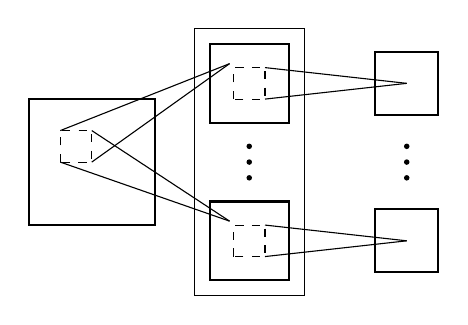
\begin{tikzpicture}
    \draw[thick] (-8mm,-8mm) rectangle (8mm,8mm);
    \draw[dashed] (-4mm, 0mm) rectangle (0mm,4mm);

    \draw[thick] (15mm,  5mm) rectangle ++(10mm,10mm);
    \foreach\y in {-2,0,2}
    {   \fill (20mm,1mm*\y) circle (1pt);
    }
    \draw[thick] (15mm,-15mm) rectangle ++(10mm,10mm);

    \draw (13mm,-17mm) rectangle (27mm,17mm);

    \draw (-4mm,4mm) -- (20mm-2.5mm, 10mm+2.5mm);
    \draw (20mm-2.5mm, 10mm+2.5mm) -- (0mm,0mm);
    \draw (0mm,4mm) -- (20mm-2.5mm,-10mm+2.5mm);
    \draw (20mm-2.5mm,-10mm+2.5mm) -- (-4mm,0mm);

    \draw[thick] (36mm, 6mm) rectangle ++(8mm,8mm);
    \foreach\y in {-2,0,2}
    {   \fill (40mm,1mm*\y) circle (1pt);
    }
    \draw[thick] (36mm,-14mm) rectangle (44mm,-6mm);

    \foreach\y in {-10,10}
    {   \draw[dashed] (18mm,1mm*\y-2mm) rectangle ++(4mm,4mm);
        \draw (22mm,1mm*\y+2mm) -- (40mm,1mm*\y);
        \draw (40mm,1mm*\y) -- (22mm,1mm*\y-2mm);
    }
\end{tikzpicture}
}
\begin{tikzpicture}
    [   kerline/.style =
        {   line join=round
        ,   densely dotted
        },
        kernel/.style =
        {   draw
        ,   circle
        ,   densely dotted
        }
    ]
    \newcommand{\kerlines}[2]{%
        \draw[kerline] (tangent cs:node=#1,point={(#2)},solution=1)
            -- (#2) -- (tangent cs:node=#1,point={(#2)},solution=2);
    }
    \newcommand{\kerdots}[1]{%
        \foreach\y in {-2,0,2}
        {   \fill (#1,1mm*\y) circle (1pt);
        }
    }

    %% planes
    % U0
    \node (U0) at ( 0mm,  0mm) [draw,rectangle,minimum size=20mm] {};
    % US1
    \node (US1G1) at (28mm,-15mm) [draw,rectangle,minimum size=16mm] {};
    \kerdots{28mm}
    \node (US1G2) at (28mm, 15mm) [draw,rectangle,minimum size=16mm] {};
    \draw (18mm,-25mm) rectangle (38mm,25mm);
    \node at (28mm,25mm) [above] {$U_{S1}$};
    % UC1
    \node (UC1G1) at (53mm,-15mm) [draw,rectangle,minimum size=14mm] {};
    \kerdots{53mm}
    \node (UC1G2)at (53mm, 15mm) [draw,rectangle,minimum size=14mm] {};
    \draw (44mm,-24mm) rectangle (62mm,24mm);
    \node at (53mm,24mm) [above] {$U_{C1}$};
    % US2
    \node (US2G1) at (75mm,-15mm) [draw,rectangle,minimum size=10mm] {};
    \kerdots{75mm}
    \node (US2G2) at (75mm, 15mm) [draw,rectangle,minimum size=10mm] {};
    \draw (68mm,-22mm) rectangle (82mm,22mm);
    \node at (75mm,22mm) [above] {$U_{S2}$};
    % UC2
    \node (UC2G1) at (94mm,-15mm) [draw,rectangle,minimum size=8mm] {};
    \kerdots{94mm}
    \node (UC2G2) at (94mm, 15mm) [draw,rectangle,minimum size=8mm] {};
    \draw (88mm,-21mm) rectangle (100mm,21mm);
    \node at (94mm,21mm) [above] {$U_{C2}$};

    %% kernels
    % U0 -> US1
    \coordinate (U0tUS1) at (-4mm,+4mm);
    \node[kernel] (U0K) at ($(U0)+(U0tUS1)$)
        [inner sep=0pt,minimum size=3mm] {};
    \coordinate (US1P1) at ($(US1G1)+(U0tUS1)$);
    \coordinate (US1P2) at ($(US1G2)+(U0tUS1)$);
    \kerlines{U0K}{US1P1}
    \kerlines{U0K}{US1P2}
    % US1 -> UC1
    \coordinate (US1tUC1) at (-4mm,-4mm);
    \node[kernel] (US1K1) at ($(US1G1)+(US1tUC1)$)
        [inner sep=0pt,minimum size=2mm] {};
    \node[kernel] (US1K2) at ($(US1G2)+(US1tUC1)$)
        [inner sep=0pt,minimum size=2mm] {};
    \coordinate (UC1P1) at ($(UC1G1)+(US1tUC1)$);
    \coordinate (UC1P2) at ($(UC1G2)+(US1tUC1)$);
    \kerlines{US1K1}{UC1P1}
    \kerlines{US1K2}{UC1P2}
    % UC1 -> US2
    \coordinate (UC1tUS2) at (-2mm,2mm);
    \node[kernel] (UC1K1) at ($(UC1G1)+(UC1tUS2)$)
        [inner sep=0pt,minimum size=3mm] {};
    \node[kernel] (UC1K2) at ($(UC1G2)+(UC1tUS2)$)
        [inner sep=0pt,minimum size=3mm] {};
    \coordinate (US2P1) at ($(US2G1)+(UC1tUS2)$);
    \coordinate (US2P2) at ($(US2G2)+(UC1tUS2)$);
    \kerlines{UC1K1}{US2P1}
    \kerlines{UC1K1}{US2P2}
    \kerlines{UC1K2}{US2P1}
    \kerlines{UC1K2}{US2P2}
    % US2 -> UC2
    \coordinate (US2tUC2) at (2mm,2mm);
    \node[kernel] (US2K1) at ($(US2G1)+(US2tUC2)$)
        [inner sep=0pt,minimum size=2mm] {};
    \node[kernel] (US2K2) at ($(US2G2)+(US2tUC2)$)
        [inner sep=0pt,minimum size=2mm] {};
    \coordinate (UC2P1) at ($(UC2G1)+(US2tUC2)$);
    \coordinate (UC2P2) at ($(UC2G2)+(US2tUC2)$);
    \kerlines{US2K1}{UC2P1}
    \kerlines{US2K2}{UC2P2}

    \foreach\x in {106,108,110}
    {   \fill (1mm*\x,0mm) circle (1pt);
    }
\end{tikzpicture}

    \captionof{figure}{Representation of the neocognitron's connectivity.}
\end{center}
Each layer of the network reduces the size of input image until the final layer
consists of single unit feature maps.
The network was originally trained to distinguish 5 digits, numbers 0 to 4,
using an unsupervised learning method, and was the first to reliably handle
shifted inputs.



\cite{Waibel:1989:Phoneme}, used concepts from the neocognitron to design the
time delay neural network, which was originally proposed for phoneme
recognition.
The networks were initially trained using backpropagation to detect and
distinguish between three acoustically similar phonemes (/b/, /d/, and /g/).
The model consisted of units similar to the neocognitron's S-Planes, where the
output of a unit is a function of a region from the previous layer.
The input for the model was a 2D spectrogram of an audio sample, with each
column representing a set of 16 spectral coefficients for a given time frame.

The first hidden layer contained columns of 8 units, each of which convolved the
spectral coefficients across 3 time frames, requiring a total of 384 weights.
Similarly, the second hidden layer contained columns of 3 units, each convolving
the previous layer across 5 time frames, requiring a total of 120 weights.
Finally, the output layer contains three units, each of which is a function of
the previous layer's corresponding row sum.
The most active unit is the phoneme present in the audio.

Once trained, the network was able to detect the correct phoneme, in real time, 
under a variety of contexts, with an error of 1.5\%, a significant improvement
over the 6.3\% error from the most popular method at the time.



% Applied to handwritten digits by \cite{LeCun:1989:Backpropagation}
% 16 by 16 pixel images, each containing one digit
% backpropagation gave better results that previous handcrafted networks
% The network took a 16 by 16 pixel image containing one digit as it's input,
% first layer convolves to create 12, 8 by 8 pixel feature maps
% second convolves to create 12, 4 by 4 pixel feature maps,
%   each only references 8 of the 12 previous layers maps
% third layer fully connected
% output fully connected
% tanh activation function
% each neuron had its own bias
Similar techniques were used by \cite{LeCun:1989:Backpropagation}, to classify
handwritten digits.
A large number of 16 by 16 pixel images were used to train a network with three
hidden layers using backpropagation.
One of the main differences that \TODO{RESUME}



% Speech recognition with max pooling \cite{Yamaguchi:1990:Neural}
% input separated into frames, $N$ is vocabulary size
% event layer, convolves data from each frame twice to produce single output
% the event layer outputs go through a pooling convolutional layer
%   that forwards the maximum value
%   exception: if all values are too low, the kernel size is increased
% word net, $W_i$, $i=1,...,N$, convolution
%   5 inputs densely to 5 hidden units to 1 output
%   trained to fire when training examples belong to group $i$, and not when not
% super net, $N$ units densely to $N+1$ hidden units to $N+1$ outputs
%   only one output active for a given input
%   output $i$ is active when word belongs to category $i$
%   output $N+1$ is active if the word could not be categorised / was rejected
% 97.1\% accuracy, 1.9\% rejected, 1.0\% error

% A Convolutional Neural Network (CNN) layer contains sets of neurons that sample
% regions of the previous layer, with all neurons within a set using the same
% weight scheme.

% The 1D case may be expressed mathematically as
% \begin{align*}
%     y_i &= \phi\left(b + \sum_{j=0}^{S} w_j x_{i+j}\right),
% \end{align*}
% where $S$ is the kernel size.
% \begin{center}
%     \begin{tikzpicture}
    [   neuron/.style=
        {   draw
        ,   circle
        ,   inner sep=2pt
        ,   node font=\small\ttfamily
        }
    ,   baseline=0pt
    ,   >={Stealth[scale=1.2]}
    ]
    \foreach\x in {0,...,3}
    {   \pgfmathtruncatemacro{\xp}{10*\x-15}
        \node[neuron] (X\x) at (2mm*\xp, 0mm) {$x_\x$};
    }
    \foreach\y in {0,...,1}
    {   \pgfmathtruncatemacro{\yp}{10*\y-5}
        \node[neuron] (Y\y) at (4mm*\yp, -20mm) {$y_\y$};
        \pgfmathtruncatemacro{\xmin}{\y}
        \pgfmathtruncatemacro{\xmax}{\y+2}
        \foreach\x in {\xmin,...,\xmax}
        {   \pgfmathtruncatemacro{\w}{\x-\xmin}
            \draw[->] (X\x) -- node[pos=0.70,inner sep=1pt,fill=white] {$w_\w$} (Y\y);
        }
    }
    %\node[neuron] (A) at ();
\end{tikzpicture}

%     \captionof{figure}{Example of a 1D CNN.}
% \end{center}
% CNNs have the advantage of encoding spacial information implicitly, which makes
% them well suited for image processing.

\subsection{RNN}
\subsection{LSTM}
